% Created by tikzDevice version 0.10.1 on 2020-02-15 16:19:10
% !TEX encoding = UTF-8 Unicode
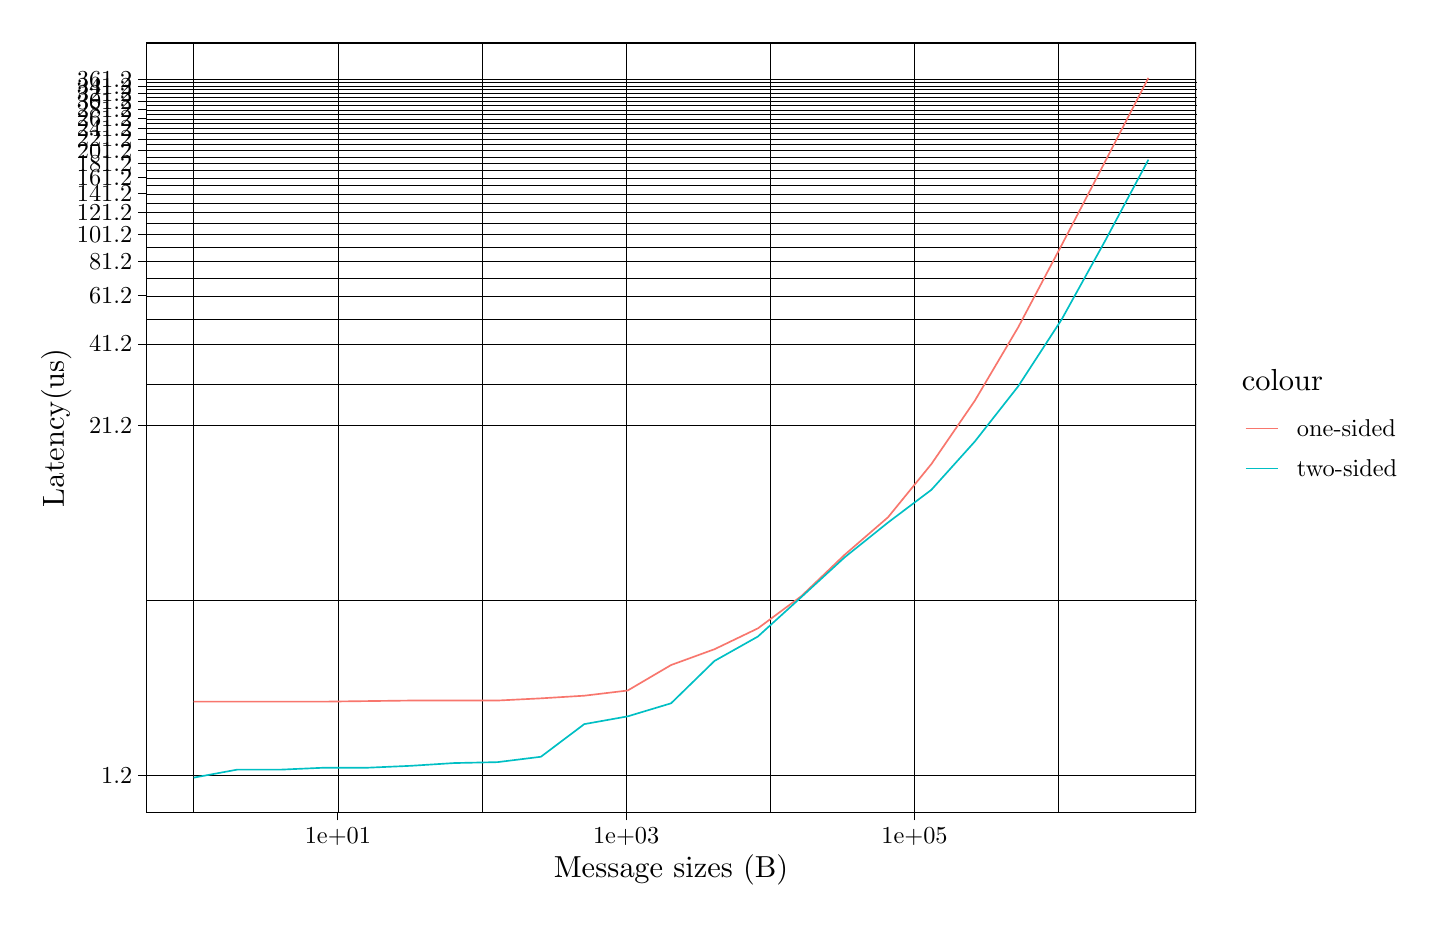
\begin{tikzpicture}[x=1pt,y=1pt]
\definecolor{fillColor}{RGB}{255,255,255}
\path[use as bounding box,fill=fillColor,fill opacity=0.00] (0,0) rectangle (505.89,314.37);
\begin{scope}
\path[clip] (  0.00,  0.00) rectangle (505.89,314.37);
\definecolor{drawColor}{RGB}{255,255,255}
\definecolor{fillColor}{RGB}{255,255,255}

\path[draw=drawColor,line width= 0.6pt,line join=round,line cap=round,fill=fillColor] (  0.00,  0.00) rectangle (505.89,314.37);
\end{scope}
\begin{scope}
\path[clip] ( 42.76, 30.72) rectangle (422.22,308.87);
\definecolor{fillColor}{RGB}{255,255,255}

\path[fill=fillColor] ( 42.76, 30.72) rectangle (422.22,308.87);
\definecolor{drawColor}{RGB}{0,0,0}

\path[draw=drawColor,line width= 0.0pt,line join=round] ( 42.76,107.41) --
	(422.22,107.41);

\path[draw=drawColor,line width= 0.0pt,line join=round] ( 42.76,185.37) --
	(422.22,185.37);

\path[draw=drawColor,line width= 0.0pt,line join=round] ( 42.76,208.74) --
	(422.22,208.74);

\path[draw=drawColor,line width= 0.0pt,line join=round] ( 42.76,223.70) --
	(422.22,223.70);

\path[draw=drawColor,line width= 0.0pt,line join=round] ( 42.76,234.78) --
	(422.22,234.78);

\path[draw=drawColor,line width= 0.0pt,line join=round] ( 42.76,243.61) --
	(422.22,243.61);

\path[draw=drawColor,line width= 0.0pt,line join=round] ( 42.76,250.96) --
	(422.22,250.96);

\path[draw=drawColor,line width= 0.0pt,line join=round] ( 42.76,257.24) --
	(422.22,257.24);

\path[draw=drawColor,line width= 0.0pt,line join=round] ( 42.76,262.74) --
	(422.22,262.74);

\path[draw=drawColor,line width= 0.0pt,line join=round] ( 42.76,267.63) --
	(422.22,267.63);

\path[draw=drawColor,line width= 0.0pt,line join=round] ( 42.76,272.03) --
	(422.22,272.03);

\path[draw=drawColor,line width= 0.0pt,line join=round] ( 42.76,276.02) --
	(422.22,276.02);

\path[draw=drawColor,line width= 0.0pt,line join=round] ( 42.76,279.69) --
	(422.22,279.69);

\path[draw=drawColor,line width= 0.0pt,line join=round] ( 42.76,283.07) --
	(422.22,283.07);

\path[draw=drawColor,line width= 0.0pt,line join=round] ( 42.76,286.21) --
	(422.22,286.21);

\path[draw=drawColor,line width= 0.0pt,line join=round] ( 42.76,289.14) --
	(422.22,289.14);

\path[draw=drawColor,line width= 0.0pt,line join=round] ( 42.76,291.89) --
	(422.22,291.89);

\path[draw=drawColor,line width= 0.0pt,line join=round] ( 42.76,294.48) --
	(422.22,294.48);

\path[draw=drawColor,line width= 0.0pt,line join=round] ( 60.01, 30.72) --
	( 60.01,308.87);

\path[draw=drawColor,line width= 0.0pt,line join=round] (164.18, 30.72) --
	(164.18,308.87);

\path[draw=drawColor,line width= 0.0pt,line join=round] (268.36, 30.72) --
	(268.36,308.87);

\path[draw=drawColor,line width= 0.0pt,line join=round] (372.54, 30.72) --
	(372.54,308.87);

\path[draw=drawColor,line width= 0.1pt,line join=round] ( 42.76, 44.11) --
	(422.22, 44.11);

\path[draw=drawColor,line width= 0.1pt,line join=round] ( 42.76,170.72) --
	(422.22,170.72);

\path[draw=drawColor,line width= 0.1pt,line join=round] ( 42.76,200.02) --
	(422.22,200.02);

\path[draw=drawColor,line width= 0.1pt,line join=round] ( 42.76,217.46) --
	(422.22,217.46);

\path[draw=drawColor,line width= 0.1pt,line join=round] ( 42.76,229.93) --
	(422.22,229.93);

\path[draw=drawColor,line width= 0.1pt,line join=round] ( 42.76,239.64) --
	(422.22,239.64);

\path[draw=drawColor,line width= 0.1pt,line join=round] ( 42.76,247.59) --
	(422.22,247.59);

\path[draw=drawColor,line width= 0.1pt,line join=round] ( 42.76,254.32) --
	(422.22,254.32);

\path[draw=drawColor,line width= 0.1pt,line join=round] ( 42.76,260.16) --
	(422.22,260.16);

\path[draw=drawColor,line width= 0.1pt,line join=round] ( 42.76,265.32) --
	(422.22,265.32);

\path[draw=drawColor,line width= 0.1pt,line join=round] ( 42.76,269.94) --
	(422.22,269.94);

\path[draw=drawColor,line width= 0.1pt,line join=round] ( 42.76,274.11) --
	(422.22,274.11);

\path[draw=drawColor,line width= 0.1pt,line join=round] ( 42.76,277.93) --
	(422.22,277.93);

\path[draw=drawColor,line width= 0.1pt,line join=round] ( 42.76,281.44) --
	(422.22,281.44);

\path[draw=drawColor,line width= 0.1pt,line join=round] ( 42.76,284.70) --
	(422.22,284.70);

\path[draw=drawColor,line width= 0.1pt,line join=round] ( 42.76,287.73) --
	(422.22,287.73);

\path[draw=drawColor,line width= 0.1pt,line join=round] ( 42.76,290.56) --
	(422.22,290.56);

\path[draw=drawColor,line width= 0.1pt,line join=round] ( 42.76,293.22) --
	(422.22,293.22);

\path[draw=drawColor,line width= 0.1pt,line join=round] ( 42.76,295.73) --
	(422.22,295.73);

\path[draw=drawColor,line width= 0.1pt,line join=round] (112.10, 30.72) --
	(112.10,308.87);

\path[draw=drawColor,line width= 0.1pt,line join=round] (216.27, 30.72) --
	(216.27,308.87);

\path[draw=drawColor,line width= 0.1pt,line join=round] (320.45, 30.72) --
	(320.45,308.87);
\definecolor{drawColor}{RGB}{248,118,109}

\path[draw=drawColor,line width= 0.6pt,line join=round] ( 60.01, 70.83) --
	( 75.69, 70.83) --
	( 91.37, 70.83) --
	(107.05, 70.83) --
	(122.73, 71.03) --
	(138.41, 71.23) --
	(154.09, 71.23) --
	(169.77, 71.23) --
	(185.45, 72.02) --
	(201.13, 72.98) --
	(216.81, 74.85) --
	(232.49, 84.06) --
	(248.17, 89.77) --
	(263.85, 97.30) --
	(279.53,108.93) --
	(295.21,123.90) --
	(310.89,137.46) --
	(326.57,156.71) --
	(342.25,179.58) --
	(357.93,206.12) --
	(373.61,235.78) --
	(389.29,265.90) --
	(404.97,296.23);
\definecolor{drawColor}{RGB}{0,191,196}

\path[draw=drawColor,line width= 0.6pt,line join=round] ( 60.01, 43.37) --
	( 75.69, 46.26) --
	( 91.37, 46.26) --
	(107.05, 46.95) --
	(122.73, 46.95) --
	(138.41, 47.64) --
	(154.09, 48.64) --
	(169.77, 48.97) --
	(185.45, 50.91) --
	(201.13, 62.71) --
	(216.81, 65.51) --
	(232.49, 70.23) --
	(248.17, 85.53) --
	(263.85, 94.35) --
	(279.53,108.59) --
	(295.21,122.98) --
	(310.89,135.56) --
	(326.57,147.39) --
	(342.25,164.83) --
	(357.93,184.79) --
	(373.61,208.91) --
	(389.29,237.27) --
	(404.97,266.66);
\definecolor{drawColor}{RGB}{0,0,0}

\path[draw=drawColor,line width= 0.6pt,line join=round,line cap=round] ( 42.76, 30.72) rectangle (422.22,308.87);
\end{scope}
\begin{scope}
\path[clip] (  0.00,  0.00) rectangle (505.89,314.37);
\definecolor{drawColor}{RGB}{0,0,0}

\node[text=drawColor,anchor=base west,inner sep=0pt, outer sep=0pt, scale=  0.88] at ( 26.57, 41.29) {1.2};

\node[text=drawColor,anchor=base west,inner sep=0pt, outer sep=0pt, scale=  0.88] at ( 22.17,167.90) {21.2};

\node[text=drawColor,anchor=base west,inner sep=0pt, outer sep=0pt, scale=  0.88] at ( 22.17,197.19) {41.2};

\node[text=drawColor,anchor=base west,inner sep=0pt, outer sep=0pt, scale=  0.88] at ( 22.17,214.64) {61.2};

\node[text=drawColor,anchor=base west,inner sep=0pt, outer sep=0pt, scale=  0.88] at ( 22.17,227.11) {81.2};

\node[text=drawColor,anchor=base west,inner sep=0pt, outer sep=0pt, scale=  0.88] at ( 17.77,236.82) {101.2};

\node[text=drawColor,anchor=base west,inner sep=0pt, outer sep=0pt, scale=  0.88] at ( 17.77,244.77) {121.2};

\node[text=drawColor,anchor=base west,inner sep=0pt, outer sep=0pt, scale=  0.88] at ( 17.77,251.50) {141.2};

\node[text=drawColor,anchor=base west,inner sep=0pt, outer sep=0pt, scale=  0.88] at ( 17.77,257.34) {161.2};

\node[text=drawColor,anchor=base west,inner sep=0pt, outer sep=0pt, scale=  0.88] at ( 17.77,262.50) {181.2};

\node[text=drawColor,anchor=base west,inner sep=0pt, outer sep=0pt, scale=  0.88] at ( 17.77,267.11) {201.2};

\node[text=drawColor,anchor=base west,inner sep=0pt, outer sep=0pt, scale=  0.88] at ( 17.77,271.29) {221.2};

\node[text=drawColor,anchor=base west,inner sep=0pt, outer sep=0pt, scale=  0.88] at ( 17.77,275.11) {241.2};

\node[text=drawColor,anchor=base west,inner sep=0pt, outer sep=0pt, scale=  0.88] at ( 17.77,278.62) {261.2};

\node[text=drawColor,anchor=base west,inner sep=0pt, outer sep=0pt, scale=  0.88] at ( 17.77,281.87) {281.2};

\node[text=drawColor,anchor=base west,inner sep=0pt, outer sep=0pt, scale=  0.88] at ( 17.77,284.90) {301.2};

\node[text=drawColor,anchor=base west,inner sep=0pt, outer sep=0pt, scale=  0.88] at ( 17.77,287.74) {321.2};

\node[text=drawColor,anchor=base west,inner sep=0pt, outer sep=0pt, scale=  0.88] at ( 17.77,290.40) {341.2};

\node[text=drawColor,anchor=base west,inner sep=0pt, outer sep=0pt, scale=  0.88] at ( 17.77,292.91) {361.2};
\end{scope}
\begin{scope}
\path[clip] (  0.00,  0.00) rectangle (505.89,314.37);
\definecolor{drawColor}{RGB}{0,0,0}

\path[draw=drawColor,line width= 0.3pt,line join=round] ( 40.01, 44.11) --
	( 42.76, 44.11);

\path[draw=drawColor,line width= 0.3pt,line join=round] ( 40.01,170.72) --
	( 42.76,170.72);

\path[draw=drawColor,line width= 0.3pt,line join=round] ( 40.01,200.02) --
	( 42.76,200.02);

\path[draw=drawColor,line width= 0.3pt,line join=round] ( 40.01,217.46) --
	( 42.76,217.46);

\path[draw=drawColor,line width= 0.3pt,line join=round] ( 40.01,229.93) --
	( 42.76,229.93);

\path[draw=drawColor,line width= 0.3pt,line join=round] ( 40.01,239.64) --
	( 42.76,239.64);

\path[draw=drawColor,line width= 0.3pt,line join=round] ( 40.01,247.59) --
	( 42.76,247.59);

\path[draw=drawColor,line width= 0.3pt,line join=round] ( 40.01,254.32) --
	( 42.76,254.32);

\path[draw=drawColor,line width= 0.3pt,line join=round] ( 40.01,260.16) --
	( 42.76,260.16);

\path[draw=drawColor,line width= 0.3pt,line join=round] ( 40.01,265.32) --
	( 42.76,265.32);

\path[draw=drawColor,line width= 0.3pt,line join=round] ( 40.01,269.94) --
	( 42.76,269.94);

\path[draw=drawColor,line width= 0.3pt,line join=round] ( 40.01,274.11) --
	( 42.76,274.11);

\path[draw=drawColor,line width= 0.3pt,line join=round] ( 40.01,277.93) --
	( 42.76,277.93);

\path[draw=drawColor,line width= 0.3pt,line join=round] ( 40.01,281.44) --
	( 42.76,281.44);

\path[draw=drawColor,line width= 0.3pt,line join=round] ( 40.01,284.70) --
	( 42.76,284.70);

\path[draw=drawColor,line width= 0.3pt,line join=round] ( 40.01,287.73) --
	( 42.76,287.73);

\path[draw=drawColor,line width= 0.3pt,line join=round] ( 40.01,290.56) --
	( 42.76,290.56);

\path[draw=drawColor,line width= 0.3pt,line join=round] ( 40.01,293.22) --
	( 42.76,293.22);

\path[draw=drawColor,line width= 0.3pt,line join=round] ( 40.01,295.73) --
	( 42.76,295.73);
\end{scope}
\begin{scope}
\path[clip] (  0.00,  0.00) rectangle (505.89,314.37);
\definecolor{drawColor}{RGB}{0,0,0}

\path[draw=drawColor,line width= 0.3pt,line join=round] (112.10, 27.97) --
	(112.10, 30.72);

\path[draw=drawColor,line width= 0.3pt,line join=round] (216.27, 27.97) --
	(216.27, 30.72);

\path[draw=drawColor,line width= 0.3pt,line join=round] (320.45, 27.97) --
	(320.45, 30.72);
\end{scope}
\begin{scope}
\path[clip] (  0.00,  0.00) rectangle (505.89,314.37);
\definecolor{drawColor}{RGB}{0,0,0}

\node[text=drawColor,anchor=base,inner sep=0pt, outer sep=0pt, scale=  0.88] at (112.10, 19.71) {1e+01};

\node[text=drawColor,anchor=base,inner sep=0pt, outer sep=0pt, scale=  0.88] at (216.27, 19.71) {1e+03};

\node[text=drawColor,anchor=base,inner sep=0pt, outer sep=0pt, scale=  0.88] at (320.45, 19.71) {1e+05};
\end{scope}
\begin{scope}
\path[clip] (  0.00,  0.00) rectangle (505.89,314.37);
\definecolor{drawColor}{RGB}{0,0,0}

\node[text=drawColor,anchor=base,inner sep=0pt, outer sep=0pt, scale=  1.10] at (232.49,  7.44) {Message sizes (B)};
\end{scope}
\begin{scope}
\path[clip] (  0.00,  0.00) rectangle (505.89,314.37);
\definecolor{drawColor}{RGB}{0,0,0}

\node[text=drawColor,rotate= 90.00,anchor=base,inner sep=0pt, outer sep=0pt, scale=  1.10] at ( 13.08,169.80) {Latency(us)};
\end{scope}
\begin{scope}
\path[clip] (  0.00,  0.00) rectangle (505.89,314.37);
\definecolor{fillColor}{RGB}{255,255,255}

\path[fill=fillColor] (433.22,142.34) rectangle (500.39,197.26);
\end{scope}
\begin{scope}
\path[clip] (  0.00,  0.00) rectangle (505.89,314.37);
\definecolor{drawColor}{RGB}{0,0,0}

\node[text=drawColor,anchor=base west,inner sep=0pt, outer sep=0pt, scale=  1.10] at (438.72,183.22) {colour};
\end{scope}
\begin{scope}
\path[clip] (  0.00,  0.00) rectangle (505.89,314.37);
\definecolor{fillColor}{RGB}{255,255,255}

\path[fill=fillColor] (438.72,162.29) rectangle (453.17,176.74);
\end{scope}
\begin{scope}
\path[clip] (  0.00,  0.00) rectangle (505.89,314.37);
\definecolor{drawColor}{RGB}{248,118,109}

\path[draw=drawColor,line width= 0.6pt,line join=round] (440.16,169.52) -- (451.73,169.52);
\end{scope}
\begin{scope}
\path[clip] (  0.00,  0.00) rectangle (505.89,314.37);
\definecolor{drawColor}{RGB}{248,118,109}

\path[draw=drawColor,line width= 0.6pt,line join=round] (440.16,169.52) -- (451.73,169.52);
\end{scope}
\begin{scope}
\path[clip] (  0.00,  0.00) rectangle (505.89,314.37);
\definecolor{fillColor}{RGB}{255,255,255}

\path[fill=fillColor] (438.72,147.84) rectangle (453.17,162.29);
\end{scope}
\begin{scope}
\path[clip] (  0.00,  0.00) rectangle (505.89,314.37);
\definecolor{drawColor}{RGB}{0,191,196}

\path[draw=drawColor,line width= 0.6pt,line join=round] (440.16,155.06) -- (451.73,155.06);
\end{scope}
\begin{scope}
\path[clip] (  0.00,  0.00) rectangle (505.89,314.37);
\definecolor{drawColor}{RGB}{0,191,196}

\path[draw=drawColor,line width= 0.6pt,line join=round] (440.16,155.06) -- (451.73,155.06);
\end{scope}
\begin{scope}
\path[clip] (  0.00,  0.00) rectangle (505.89,314.37);
\definecolor{drawColor}{RGB}{0,0,0}

\node[text=drawColor,anchor=base west,inner sep=0pt, outer sep=0pt, scale=  0.88] at (458.67,166.49) {one-sided};
\end{scope}
\begin{scope}
\path[clip] (  0.00,  0.00) rectangle (505.89,314.37);
\definecolor{drawColor}{RGB}{0,0,0}

\node[text=drawColor,anchor=base west,inner sep=0pt, outer sep=0pt, scale=  0.88] at (458.67,152.03) {two-sided};
\end{scope}
\end{tikzpicture}
